\documentclass[1p]{elsarticle_modified}
%\bibliographystyle{elsarticle-num}

%\usepackage[colorlinks]{hyperref}
%\usepackage{abbrmath_seonhwa} %\Abb, \Ascr, \Acal ,\Abf, \Afrak
\usepackage{amsfonts}
\usepackage{amssymb}
\usepackage{amsmath}
\usepackage{amsthm}
\usepackage{scalefnt}
\usepackage{amsbsy}
\usepackage{kotex}
\usepackage{caption}
\usepackage{subfig}
\usepackage{color}
\usepackage{graphicx}
\usepackage{xcolor} %% white, black, red, green, blue, cyan, magenta, yellow
\usepackage{float}
\usepackage{setspace}
\usepackage{hyperref}

\usepackage{tikz}
\usetikzlibrary{arrows}

\usepackage{multirow}
\usepackage{array} % fixed length table
\usepackage{hhline}

%%%%%%%%%%%%%%%%%%%%%
\makeatletter
\renewcommand*\env@matrix[1][\arraystretch]{%
	\edef\arraystretch{#1}%
	\hskip -\arraycolsep
	\let\@ifnextchar\new@ifnextchar
	\array{*\c@MaxMatrixCols c}}
\makeatother %https://tex.stackexchange.com/questions/14071/how-can-i-increase-the-line-spacing-in-a-matrix
%%%%%%%%%%%%%%%

\usepackage[normalem]{ulem}

\newcommand{\msout}[1]{\ifmmode\text{\sout{\ensuremath{#1}}}\else\sout{#1}\fi}
%SOURCE: \msout is \stkout macro in https://tex.stackexchange.com/questions/20609/strikeout-in-math-mode

\newcommand{\cancel}[1]{
	\ifmmode
	{\color{red}\msout{#1}}
	\else
	{\color{red}\sout{#1}}
	\fi
}

\newcommand{\add}[1]{
	{\color{blue}\uwave{#1}}
}

\newcommand{\replace}[2]{
	\ifmmode
	{\color{red}\msout{#1}}{\color{blue}\uwave{#2}}
	\else
	{\color{red}\sout{#1}}{\color{blue}\uwave{#2}}
	\fi
}

\newcommand{\Sol}{\mathcal{S}} %segment
\newcommand{\D}{D} %diagram
\newcommand{\A}{\mathcal{A}} %arc


%%%%%%%%%%%%%%%%%%%%%%%%%%%%%5 test

\def\sl{\operatorname{\textup{SL}}(2,\Cbb)}
\def\psl{\operatorname{\textup{PSL}}(2,\Cbb)}
\def\quan{\mkern 1mu \triangleright \mkern 1mu}

\theoremstyle{definition}
\newtheorem{thm}{Theorem}[section]
\newtheorem{prop}[thm]{Proposition}
\newtheorem{lem}[thm]{Lemma}
\newtheorem{ques}[thm]{Question}
\newtheorem{cor}[thm]{Corollary}
\newtheorem{defn}[thm]{Definition}
\newtheorem{exam}[thm]{Example}
\newtheorem{rmk}[thm]{Remark}
\newtheorem{alg}[thm]{Algorithm}

\newcommand{\I}{\sqrt{-1}}
\begin{document}

%\begin{frontmatter}
%
%\title{Boundary parabolic representations of knots up to 8 crossings}
%
%%% Group authors per affiliation:
%\author{Yunhi Cho} 
%\address{Department of Mathematics, University of Seoul, Seoul, Korea}
%\ead{yhcho@uos.ac.kr}
%
%
%\author{Seonhwa Kim} %\fnref{s_kim}}
%\address{Center for Geometry and Physics, Institute for Basic Science, Pohang, 37673, Korea}
%\ead{ryeona17@ibs.re.kr}
%
%\author{Hyuk Kim}
%\address{Department of Mathematical Sciences, Seoul National University, Seoul 08826, Korea}
%\ead{hyukkim@snu.ac.kr}
%
%\author{Seokbeom Yoon}
%\address{Department of Mathematical Sciences, Seoul National University, Seoul, 08826,  Korea}
%\ead{sbyoon15@snu.ac.kr}
%
%\begin{abstract}
%We find all boundary parabolic representation of knots up to 8 crossings.
%
%\end{abstract}
%\begin{keyword}
%    \MSC[2010] 57M25 
%\end{keyword}
%
%\end{frontmatter}

%\linenumbers
%\tableofcontents
%
\newcommand\colored[1]{\textcolor{white}{\rule[-0.35ex]{0.8em}{1.4ex}}\kern-0.8em\color{red} #1}%
%\newcommand\colored[1]{\textcolor{white}{ #1}\kern-2.17ex	\textcolor{white}{ #1}\kern-1.81ex	\textcolor{white}{ #1}\kern-2.15ex\color{red}#1	}

{\Large $\underline{12n_{0023}~(K12n_{0023})}$}

\setlength{\tabcolsep}{10pt}
\renewcommand{\arraystretch}{1.6}
\vspace{1cm}\begin{tabular}{m{100pt}>{\centering\arraybackslash}m{274pt}}
\multirow{5}{120pt}{
	\centering
	\includegraphics[width=112pt]{../../../GIT/diagram.site/Diagrams/png/2112_12n_0023.png}\\
\ \ \ A knot diagram\footnotemark}&
\allowdisplaybreaks
\textbf{Linearized knot diagam} \\
\cline{2-2}
 &
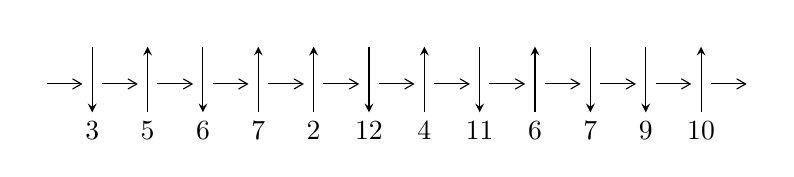
\begin{tikzpicture}[x=20pt, y=17pt]
	% nodes
	\node (C0) at (0, 0) {};
	\node (C1) at (1, 0) {};
	\node (C1U) at (1, +1) {};
	\node (C1D) at (1, -1) {3};

	\node (C2) at (2, 0) {};
	\node (C2U) at (2, +1) {};
	\node (C2D) at (2, -1) {5};

	\node (C3) at (3, 0) {};
	\node (C3U) at (3, +1) {};
	\node (C3D) at (3, -1) {6};

	\node (C4) at (4, 0) {};
	\node (C4U) at (4, +1) {};
	\node (C4D) at (4, -1) {7};

	\node (C5) at (5, 0) {};
	\node (C5U) at (5, +1) {};
	\node (C5D) at (5, -1) {2};

	\node (C6) at (6, 0) {};
	\node (C6U) at (6, +1) {};
	\node (C6D) at (6, -1) {12};

	\node (C7) at (7, 0) {};
	\node (C7U) at (7, +1) {};
	\node (C7D) at (7, -1) {4};

	\node (C8) at (8, 0) {};
	\node (C8U) at (8, +1) {};
	\node (C8D) at (8, -1) {11};

	\node (C9) at (9, 0) {};
	\node (C9U) at (9, +1) {};
	\node (C9D) at (9, -1) {6};

	\node (C10) at (10, 0) {};
	\node (C10U) at (10, +1) {};
	\node (C10D) at (10, -1) {7};

	\node (C11) at (11, 0) {};
	\node (C11U) at (11, +1) {};
	\node (C11D) at (11, -1) {9};

	\node (C12) at (12, 0) {};
	\node (C12U) at (12, +1) {};
	\node (C12D) at (12, -1) {10};
	\node (C13) at (13, 0) {};

	% arrows
	\draw[->,>={angle 60}]
	(C0) edge (C1) (C1) edge (C2) (C2) edge (C3) (C3) edge (C4) (C4) edge (C5) (C5) edge (C6) (C6) edge (C7) (C7) edge (C8) (C8) edge (C9) (C9) edge (C10) (C10) edge (C11) (C11) edge (C12) (C12) edge (C13) ;	\draw[->,>=stealth]
	(C1U) edge (C1D) (C2D) edge (C2U) (C3U) edge (C3D) (C4D) edge (C4U) (C5D) edge (C5U) (C6U) edge (C6D) (C7D) edge (C7U) (C8U) edge (C8D) (C9D) edge (C9U) (C10U) edge (C10D) (C11U) edge (C11D) (C12D) edge (C12U) ;
	\end{tikzpicture} \\
\hhline{~~} \\& 
\textbf{Solving Sequence} \\ \cline{2-2} 
 &
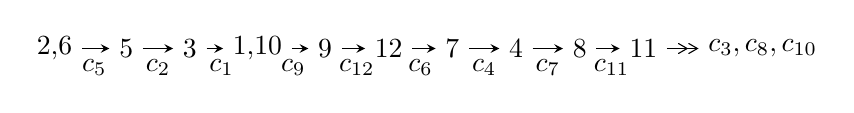
\begin{tikzpicture}[x=23pt, y=7pt]
	% node
	\node (A0) at (-1/8, 0) {2,6};
	\node (A1) at (1, 0) {5};
	\node (A2) at (2, 0) {3};
	\node (A3) at (49/16, 0) {1,10};
	\node (A4) at (33/8, 0) {9};
	\node (A5) at (41/8, 0) {12};
	\node (A6) at (49/8, 0) {7};
	\node (A7) at (57/8, 0) {4};
	\node (A8) at (65/8, 0) {8};
	\node (A9) at (73/8, 0) {11};
	\node (C1) at (1/2, -1) {$c_{5}$};
	\node (C2) at (3/2, -1) {$c_{2}$};
	\node (C3) at (5/2, -1) {$c_{1}$};
	\node (C4) at (29/8, -1) {$c_{9}$};
	\node (C5) at (37/8, -1) {$c_{12}$};
	\node (C6) at (45/8, -1) {$c_{6}$};
	\node (C7) at (53/8, -1) {$c_{4}$};
	\node (C8) at (61/8, -1) {$c_{7}$};
	\node (C9) at (69/8, -1) {$c_{11}$};
	\node (A10) at (11, 0) {$c_{3},c_{8},c_{10}$};

	% edge
	\draw[->,>=stealth]	
	(A0) edge (A1) (A1) edge (A2) (A2) edge (A3) (A3) edge (A4) (A4) edge (A5) (A5) edge (A6) (A6) edge (A7) (A7) edge (A8) (A8) edge (A9) ;
	\draw[->>,>={angle 60}]	
	(A9) edge (A10);
\end{tikzpicture} \\ 

\end{tabular} \\

\footnotetext{
The image of knot diagram is generated by the software ``\textbf{Draw programme}" developed by Andrew Bartholomew(\url{http://www.layer8.co.uk/maths/draw/index.htm\#Running-draw}), where we modified some parts for our purpose(\url{https://github.com/CATsTAILs/LinksPainter}).
}\phantom \\ \newline 
\centering \textbf{Ideals for irreducible components\footnotemark of $X_{\text{par}}$} 
 
\begin{align*}
I^u_{1}&=\langle 
-65383723517 u^{23}-453837508340 u^{22}+\cdots+211475563064 b-190647925896,\\
\phantom{I^u_{1}}&\phantom{= \langle  }-283168958672 u^{23}-1828538327515 u^{22}+\cdots+422951126128 a-1427493398353,\\
\phantom{I^u_{1}}&\phantom{= \langle  }u^{24}+7 u^{23}+\cdots+4 u+1\rangle \\
I^u_{2}&=\langle 
- u^3- u^2+b- u,\;- u^3+a- u+1,\;u^4+u^2- u+1\rangle \\
I^u_{3}&=\langle 
85 a^4 u-127 a^4+387 a^3 u-586 a^3+170 a^2 u-254 a^2-1331 a u+661 b+690 a-639 u+76,\\
\phantom{I^u_{3}}&\phantom{= \langle  }a^5+a^4 u+5 a^4+3 a^3 u+4 a^3+4 a^2 u-6 a^2+4 a u-7 a+3 u-1,\;u^2- u+1\rangle \\
I^u_{4}&=\langle 
- u^5- u^4-2 u^3- u^2+b- u-1,\;- u^3-2 u^2+a-2 u-1,\;u^6+u^5+2 u^4+2 u^3+2 u^2+2 u+1\rangle \\
\\
\end{align*}
\raggedright * 4 irreducible components of $\dim_{\mathbb{C}}=0$, with total 44 representations.\\
\footnotetext{All coefficients of polynomials are rational numbers. But the coefficients are sometimes approximated in decimal forms when there is not enough margin.}
\newpage
\renewcommand{\arraystretch}{1}
\centering \section*{I. $I^u_{1}= \langle -6.54\times10^{10} u^{23}-4.54\times10^{11} u^{22}+\cdots+2.11\times10^{11} b-1.91\times10^{11},\;-2.83\times10^{11} u^{23}-1.83\times10^{12} u^{22}+\cdots+4.23\times10^{11} a-1.43\times10^{12},\;u^{24}+7 u^{23}+\cdots+4 u+1 \rangle$}
\flushleft \textbf{(i) Arc colorings}\\
\begin{tabular}{m{7pt} m{180pt} m{7pt} m{180pt} }
\flushright $a_{2}=$&$\begin{pmatrix}0\\u\end{pmatrix}$ \\
\flushright $a_{6}=$&$\begin{pmatrix}1\\0\end{pmatrix}$ \\
\flushright $a_{5}=$&$\begin{pmatrix}1\\u^2\end{pmatrix}$ \\
\flushright $a_{3}=$&$\begin{pmatrix}u\\u^3+u\end{pmatrix}$ \\
\flushright $a_{1}=$&$\begin{pmatrix}u^3\\u^5+u^3+u\end{pmatrix}$ \\
\flushright $a_{10}=$&$\begin{pmatrix}0.669508 u^{23}+4.32329 u^{22}+\cdots-0.711116 u+3.37508\\0.309179 u^{23}+2.14605 u^{22}+\cdots+1.09437 u+0.901513\end{pmatrix}$ \\
\flushright $a_{9}=$&$\begin{pmatrix}0.360329 u^{23}+2.17723 u^{22}+\cdots-1.80549 u+2.47357\\0.309179 u^{23}+2.14605 u^{22}+\cdots+1.09437 u+0.901513\end{pmatrix}$ \\
\flushright $a_{12}=$&$\begin{pmatrix}0.954675 u^{23}+6.60431 u^{22}+\cdots+5.13017 u+0.682204\\0.103867 u^{23}+0.631846 u^{22}+\cdots+1.92070 u+0.466780\end{pmatrix}$ \\
\flushright $a_{7}=$&$\begin{pmatrix}-0.379476 u^{23}-2.46625 u^{22}+\cdots-1.86572 u-1.71578\\-0.260086 u^{23}-1.75059 u^{22}+\cdots-0.202905 u-0.639562\end{pmatrix}$ \\
\flushright $a_{4}=$&$\begin{pmatrix}- u^3\\u^3+u\end{pmatrix}$ \\
\flushright $a_{8}=$&$\begin{pmatrix}-0.336233 u^{23}-2.26307 u^{22}+\cdots-1.85658 u-1.73341\\-0.223668 u^{23}-1.41378 u^{22}+\cdots+0.416575 u-0.352405\end{pmatrix}$ \\
\flushright $a_{11}=$&$\begin{pmatrix}0.406427 u^{23}+2.72175 u^{22}+\cdots-0.116545 u+1.59093\\0.178954 u^{23}+1.12467 u^{22}+\cdots+1.69860 u+0.508208\end{pmatrix}$\\&\end{tabular}
\flushleft \textbf{(ii) Obstruction class $= -1$}\\~\\
\flushleft \textbf{(iii) Cusp Shapes $= -\frac{372525508513}{422951126128} u^{23}-\frac{297894180927}{52868890766} u^{22}+\cdots-\frac{5224084603407}{422951126128} u-\frac{308570800851}{52868890766}$}\\~\\
\newpage\renewcommand{\arraystretch}{1}
\flushleft \textbf{(iv) u-Polynomials at the component}\newline \\
\begin{tabular}{m{50pt}|m{274pt}}
Crossings & \hspace{64pt}u-Polynomials at each crossing \\
\hline $$\begin{aligned}c_{1}\end{aligned}$$&$\begin{aligned}
&u^{24}+3 u^{23}+\cdots-8 u+1
\end{aligned}$\\
\hline $$\begin{aligned}c_{2},c_{5}\end{aligned}$$&$\begin{aligned}
&u^{24}+7 u^{23}+\cdots+4 u+1
\end{aligned}$\\
\hline $$\begin{aligned}c_{3}\end{aligned}$$&$\begin{aligned}
&u^{24}-7 u^{23}+\cdots+155372 u+47236
\end{aligned}$\\
\hline $$\begin{aligned}c_{4},c_{7}\end{aligned}$$&$\begin{aligned}
&u^{24}+2 u^{23}+\cdots+7168 u+1024
\end{aligned}$\\
\hline $$\begin{aligned}c_{6}\end{aligned}$$&$\begin{aligned}
&u^{24}-4 u^{23}+\cdots-3 u+1
\end{aligned}$\\
\hline $$\begin{aligned}c_{8},c_{11}\end{aligned}$$&$\begin{aligned}
&u^{24}-13 u^{23}+\cdots-2 u+1
\end{aligned}$\\
\hline $$\begin{aligned}c_{9}\end{aligned}$$&$\begin{aligned}
&u^{24}-2 u^{23}+\cdots+2185 u+1831
\end{aligned}$\\
\hline $$\begin{aligned}c_{10}\end{aligned}$$&$\begin{aligned}
&u^{24}+4 u^{23}+\cdots-3009503 u+1672193
\end{aligned}$\\
\hline $$\begin{aligned}c_{12}\end{aligned}$$&$\begin{aligned}
&u^{24}+u^{23}+\cdots-5120 u+1024
\end{aligned}$\\
\hline
\end{tabular}\\~\\
\newpage\renewcommand{\arraystretch}{1}
\flushleft \textbf{(v) Riley Polynomials at the component}\newline \\
\begin{tabular}{m{50pt}|m{274pt}}
Crossings & \hspace{64pt}Riley Polynomials at each crossing \\
\hline $$\begin{aligned}c_{1}\end{aligned}$$&$\begin{aligned}
&y^{24}+43 y^{23}+\cdots+60 y+1
\end{aligned}$\\
\hline $$\begin{aligned}c_{2},c_{5}\end{aligned}$$&$\begin{aligned}
&y^{24}+3 y^{23}+\cdots-8 y+1
\end{aligned}$\\
\hline $$\begin{aligned}c_{3}\end{aligned}$$&$\begin{aligned}
&y^{24}+107 y^{23}+\cdots-359116296 y+2231239696
\end{aligned}$\\
\hline $$\begin{aligned}c_{4},c_{7}\end{aligned}$$&$\begin{aligned}
&y^{24}-30 y^{23}+\cdots-3145728 y+1048576
\end{aligned}$\\
\hline $$\begin{aligned}c_{6}\end{aligned}$$&$\begin{aligned}
&y^{24}+30 y^{22}+\cdots+y+1
\end{aligned}$\\
\hline $$\begin{aligned}c_{8},c_{11}\end{aligned}$$&$\begin{aligned}
&y^{24}-27 y^{23}+\cdots-198 y+1
\end{aligned}$\\
\hline $$\begin{aligned}c_{9}\end{aligned}$$&$\begin{aligned}
&y^{24}+20 y^{23}+\cdots+72680737 y+3352561
\end{aligned}$\\
\hline $$\begin{aligned}c_{10}\end{aligned}$$&$\begin{aligned}
&y^{24}+132 y^{23}+\cdots+20945455419869 y+2796229429249
\end{aligned}$\\
\hline $$\begin{aligned}c_{12}\end{aligned}$$&$\begin{aligned}
&y^{24}-57 y^{23}+\cdots-1572864 y+1048576
\end{aligned}$\\
\hline
\end{tabular}\\~\\
\newpage\flushleft \textbf{(vi) Complex Volumes and Cusp Shapes}
$$\begin{array}{c|c|c}  
\text{Solutions to }I^u_{1}& \I (\text{vol} + \sqrt{-1}CS) & \text{Cusp shape}\\
 \hline 
\begin{aligned}
u &= \phantom{-}0.389764 + 0.874669 I \\
a &= -2.77917 - 3.58598 I \\
b &= \phantom{-}0.772730 + 0.886269 I\end{aligned}
 & -2.26240 + 2.45863 I & -0.58956 - 2.80745 I \\ \hline\begin{aligned}
u &= \phantom{-}0.389764 - 0.874669 I \\
a &= -2.77917 + 3.58598 I \\
b &= \phantom{-}0.772730 - 0.886269 I\end{aligned}
 & -2.26240 - 2.45863 I & -0.58956 + 2.80745 I \\ \hline\begin{aligned}
u &= \phantom{-}0.531670 + 0.965706 I \\
a &= -1.110060 - 0.431467 I \\
b &= \phantom{-}0.161827 - 0.572669 I\end{aligned}
 & -0.14272 + 2.78886 I & \phantom{-}1.24898 - 0.91559 I \\ \hline\begin{aligned}
u &= \phantom{-}0.531670 - 0.965706 I \\
a &= -1.110060 + 0.431467 I \\
b &= \phantom{-}0.161827 + 0.572669 I\end{aligned}
 & -0.14272 - 2.78886 I & \phantom{-}1.24898 + 0.91559 I \\ \hline\begin{aligned}
u &= \phantom{-}0.476195 + 0.627959 I \\
a &= -0.327508 + 0.824390 I \\
b &= \phantom{-}0.002656 + 0.357569 I\end{aligned}
 & \phantom{-}0.84077 + 1.37467 I & \phantom{-}5.35239 - 4.26754 I \\ \hline\begin{aligned}
u &= \phantom{-}0.476195 - 0.627959 I \\
a &= -0.327508 - 0.824390 I \\
b &= \phantom{-}0.002656 - 0.357569 I\end{aligned}
 & \phantom{-}0.84077 - 1.37467 I & \phantom{-}5.35239 + 4.26754 I \\ \hline\begin{aligned}
u &= -0.686903 + 1.011450 I \\
a &= -0.675553 - 0.075442 I \\
b &= \phantom{-}0.016958 + 1.263390 I\end{aligned}
 & -5.30004 - 7.06597 I & -3.39619 + 6.37751 I \\ \hline\begin{aligned}
u &= -0.686903 - 1.011450 I \\
a &= -0.675553 + 0.075442 I \\
b &= \phantom{-}0.016958 - 1.263390 I\end{aligned}
 & -5.30004 + 7.06597 I & -3.39619 - 6.37751 I \\ \hline\begin{aligned}
u &= -0.539649 + 1.181310 I \\
a &= \phantom{-}0.959620 - 0.350796 I \\
b &= -1.16629 - 1.15098 I\end{aligned}
 & -5.91731 + 1.32680 I & -4.55064 - 0.68264 I \\ \hline\begin{aligned}
u &= -0.539649 - 1.181310 I \\
a &= \phantom{-}0.959620 + 0.350796 I \\
b &= -1.16629 + 1.15098 I\end{aligned}
 & -5.91731 - 1.32680 I & -4.55064 + 0.68264 I\\
 \hline 
 \end{array}$$\newpage$$\begin{array}{c|c|c}  
\text{Solutions to }I^u_{1}& \I (\text{vol} + \sqrt{-1}CS) & \text{Cusp shape}\\
 \hline 
\begin{aligned}
u &= \phantom{-}1.064580 + 0.846503 I \\
a &= -0.62366 - 1.42540 I \\
b &= \phantom{-}1.03585 - 3.55889 I\end{aligned}
 & \phantom{-}0.03963 + 1.93559 I & \phantom{-}3.24137 - 4.51519 I \\ \hline\begin{aligned}
u &= \phantom{-}1.064580 - 0.846503 I \\
a &= -0.62366 + 1.42540 I \\
b &= \phantom{-}1.03585 + 3.55889 I\end{aligned}
 & \phantom{-}0.03963 - 1.93559 I & \phantom{-}3.24137 + 4.51519 I \\ \hline\begin{aligned}
u &= -0.89305 + 1.24747 I \\
a &= -1.03439 - 1.00571 I \\
b &= -1.51651 + 1.14075 I\end{aligned}
 & \phantom{-}13.6003 - 6.5164 I & -1.83375 + 2.31506 I \\ \hline\begin{aligned}
u &= -0.89305 - 1.24747 I \\
a &= -1.03439 + 1.00571 I \\
b &= -1.51651 - 1.14075 I\end{aligned}
 & \phantom{-}13.6003 + 6.5164 I & -1.83375 - 2.31506 I \\ \hline\begin{aligned}
u &= -0.87342 + 1.29253 I \\
a &= \phantom{-}1.44913 + 1.22589 I \\
b &= \phantom{-}1.70664 - 2.23520 I\end{aligned}
 & \phantom{-}13.5215 - 14.1664 I & -1.97832 + 6.01811 I \\ \hline\begin{aligned}
u &= -0.87342 - 1.29253 I \\
a &= \phantom{-}1.44913 - 1.22589 I \\
b &= \phantom{-}1.70664 + 2.23520 I\end{aligned}
 & \phantom{-}13.5215 + 14.1664 I & -1.97832 - 6.01811 I \\ \hline\begin{aligned}
u &= -1.38451 + 0.86873 I \\
a &= -0.750407 - 0.670749 I \\
b &= -2.63229 - 0.87469 I\end{aligned}
 & \phantom{-}15.2941 - 1.5620 I & -0.87276 + 1.81859 I \\ \hline\begin{aligned}
u &= -1.38451 - 0.86873 I \\
a &= -0.750407 + 0.670749 I \\
b &= -2.63229 + 0.87469 I\end{aligned}
 & \phantom{-}15.2941 + 1.5620 I & -0.87276 - 1.81859 I \\ \hline\begin{aligned}
u &= -1.48666 + 0.74894 I \\
a &= \phantom{-}0.372127 + 0.956988 I \\
b &= \phantom{-}2.70664 + 2.90079 I\end{aligned}
 & \phantom{-}15.6939 + 6.0170 I & -0.56934 - 2.21062 I \\ \hline\begin{aligned}
u &= -1.48666 - 0.74894 I \\
a &= \phantom{-}0.372127 - 0.956988 I \\
b &= \phantom{-}2.70664 - 2.90079 I\end{aligned}
 & \phantom{-}15.6939 - 6.0170 I & -0.56934 + 2.21062 I\\
 \hline 
 \end{array}$$\newpage$$\begin{array}{c|c|c}  
\text{Solutions to }I^u_{1}& \I (\text{vol} + \sqrt{-1}CS) & \text{Cusp shape}\\
 \hline 
\begin{aligned}
u &= \phantom{-}0.166881 + 0.257157 I \\
a &= \phantom{-}2.61727 - 2.58686 I \\
b &= -0.422595 + 0.308191 I\end{aligned}
 & -2.60162 - 0.06406 I & -5.33602 - 1.30009 I \\ \hline\begin{aligned}
u &= \phantom{-}0.166881 - 0.257157 I \\
a &= \phantom{-}2.61727 + 2.58686 I \\
b &= -0.422595 - 0.308191 I\end{aligned}
 & -2.60162 + 0.06406 I & -5.33602 + 1.30009 I \\ \hline\begin{aligned}
u &= -0.264909 + 0.086925 I \\
a &= \phantom{-}0.90260 + 2.62839 I \\
b &= \phantom{-}0.334375 + 0.643835 I\end{aligned}
 & \phantom{-}0.00212 + 1.46917 I & \phantom{-}0.28384 - 4.39333 I \\ \hline\begin{aligned}
u &= -0.264909 - 0.086925 I \\
a &= \phantom{-}0.90260 - 2.62839 I \\
b &= \phantom{-}0.334375 - 0.643835 I\end{aligned}
 & \phantom{-}0.00212 - 1.46917 I & \phantom{-}0.28384 + 4.39333 I\\
 \hline 
 \end{array}$$\newpage\newpage\renewcommand{\arraystretch}{1}
\centering \section*{II. $I^u_{2}= \langle - u^3- u^2+b- u,\;- u^3+a- u+1,\;u^4+u^2- u+1 \rangle$}
\flushleft \textbf{(i) Arc colorings}\\
\begin{tabular}{m{7pt} m{180pt} m{7pt} m{180pt} }
\flushright $a_{2}=$&$\begin{pmatrix}0\\u\end{pmatrix}$ \\
\flushright $a_{6}=$&$\begin{pmatrix}1\\0\end{pmatrix}$ \\
\flushright $a_{5}=$&$\begin{pmatrix}1\\u^2\end{pmatrix}$ \\
\flushright $a_{3}=$&$\begin{pmatrix}u\\u^3+u\end{pmatrix}$ \\
\flushright $a_{1}=$&$\begin{pmatrix}u^3\\u^2\end{pmatrix}$ \\
\flushright $a_{10}=$&$\begin{pmatrix}u^3+u-1\\u^3+u^2+u\end{pmatrix}$ \\
\flushright $a_{9}=$&$\begin{pmatrix}- u^2-1\\u^3+u^2+u\end{pmatrix}$ \\
\flushright $a_{12}=$&$\begin{pmatrix}u^3\\u^2\end{pmatrix}$ \\
\flushright $a_{7}=$&$\begin{pmatrix}- u^3+u^2- u+1\\- u^2+u-1\end{pmatrix}$ \\
\flushright $a_{4}=$&$\begin{pmatrix}- u^3\\u^3+u\end{pmatrix}$ \\
\flushright $a_{8}=$&$\begin{pmatrix}- u^3\\- u^2\end{pmatrix}$ \\
\flushright $a_{11}=$&$\begin{pmatrix}u^3- u^2-1\\u^3+2 u^2+u\end{pmatrix}$\\&\end{tabular}
\flushleft \textbf{(ii) Obstruction class $= 1$}\\~\\
\flushleft \textbf{(iii) Cusp Shapes $= u^3-6 u^2+2 u-7$}\\~\\
\newpage\renewcommand{\arraystretch}{1}
\flushleft \textbf{(iv) u-Polynomials at the component}\newline \\
\begin{tabular}{m{50pt}|m{274pt}}
Crossings & \hspace{64pt}u-Polynomials at each crossing \\
\hline $$\begin{aligned}c_{1}\end{aligned}$$&$\begin{aligned}
&u^4-2 u^3+3 u^2- u+1
\end{aligned}$\\
\hline $$\begin{aligned}c_{2},c_{4}\end{aligned}$$&$\begin{aligned}
&u^4+u^2+u+1
\end{aligned}$\\
\hline $$\begin{aligned}c_{3}\end{aligned}$$&$\begin{aligned}
&u^4+3 u^3+4 u^2+3 u+2
\end{aligned}$\\
\hline $$\begin{aligned}c_{5},c_{7}\end{aligned}$$&$\begin{aligned}
&u^4+u^2- u+1
\end{aligned}$\\
\hline $$\begin{aligned}c_{6}\end{aligned}$$&$\begin{aligned}
&u^4+2 u^3+3 u^2+u+1
\end{aligned}$\\
\hline $$\begin{aligned}c_{8}\end{aligned}$$&$\begin{aligned}
&(u-1)^4
\end{aligned}$\\
\hline $$\begin{aligned}c_{9},c_{10}\end{aligned}$$&$\begin{aligned}
&u^4+u^3+3 u^2+2 u+1
\end{aligned}$\\
\hline $$\begin{aligned}c_{11}\end{aligned}$$&$\begin{aligned}
&(u+1)^4
\end{aligned}$\\
\hline $$\begin{aligned}c_{12}\end{aligned}$$&$\begin{aligned}
&u^4
\end{aligned}$\\
\hline
\end{tabular}\\~\\
\newpage\renewcommand{\arraystretch}{1}
\flushleft \textbf{(v) Riley Polynomials at the component}\newline \\
\begin{tabular}{m{50pt}|m{274pt}}
Crossings & \hspace{64pt}Riley Polynomials at each crossing \\
\hline $$\begin{aligned}c_{1},c_{6}\end{aligned}$$&$\begin{aligned}
&y^4+2 y^3+7 y^2+5 y+1
\end{aligned}$\\
\hline $$\begin{aligned}c_{2},c_{4},c_{5}\\c_{7}\end{aligned}$$&$\begin{aligned}
&y^4+2 y^3+3 y^2+y+1
\end{aligned}$\\
\hline $$\begin{aligned}c_{3}\end{aligned}$$&$\begin{aligned}
&y^4- y^3+2 y^2+7 y+4
\end{aligned}$\\
\hline $$\begin{aligned}c_{8},c_{11}\end{aligned}$$&$\begin{aligned}
&(y-1)^4
\end{aligned}$\\
\hline $$\begin{aligned}c_{9},c_{10}\end{aligned}$$&$\begin{aligned}
&y^4+5 y^3+7 y^2+2 y+1
\end{aligned}$\\
\hline $$\begin{aligned}c_{12}\end{aligned}$$&$\begin{aligned}
&y^4
\end{aligned}$\\
\hline
\end{tabular}\\~\\
\newpage\flushleft \textbf{(vi) Complex Volumes and Cusp Shapes}
$$\begin{array}{c|c|c}  
\text{Solutions to }I^u_{2}& \I (\text{vol} + \sqrt{-1}CS) & \text{Cusp shape}\\
 \hline 
\begin{aligned}
u &= \phantom{-}0.547424 + 0.585652 I \\
a &= -0.851808 + 0.911292 I \\
b &= \phantom{-}0.10488 + 1.55249 I\end{aligned}
 & -0.66484 + 1.39709 I & -6.04449 - 2.35025 I \\ \hline\begin{aligned}
u &= \phantom{-}0.547424 - 0.585652 I \\
a &= -0.851808 - 0.911292 I \\
b &= \phantom{-}0.10488 - 1.55249 I\end{aligned}
 & -0.66484 - 1.39709 I & -6.04449 + 2.35025 I \\ \hline\begin{aligned}
u &= -0.547424 + 1.120870 I \\
a &= \phantom{-}0.351808 + 0.720342 I \\
b &= \phantom{-}0.395123 - 0.506844 I\end{aligned}
 & -4.26996 - 7.64338 I & -0.45551 + 9.20433 I \\ \hline\begin{aligned}
u &= -0.547424 - 1.120870 I \\
a &= \phantom{-}0.351808 - 0.720342 I \\
b &= \phantom{-}0.395123 + 0.506844 I\end{aligned}
 & -4.26996 + 7.64338 I & -0.45551 - 9.20433 I\\
 \hline 
 \end{array}$$\newpage\newpage\renewcommand{\arraystretch}{1}
\centering \section*{III. $I^u_{3}= \langle 85 a^4 u+387 a^3 u+\cdots+690 a+76,\;a^4 u+3 a^3 u+\cdots-7 a-1,\;u^2- u+1 \rangle$}
\flushleft \textbf{(i) Arc colorings}\\
\begin{tabular}{m{7pt} m{180pt} m{7pt} m{180pt} }
\flushright $a_{2}=$&$\begin{pmatrix}0\\u\end{pmatrix}$ \\
\flushright $a_{6}=$&$\begin{pmatrix}1\\0\end{pmatrix}$ \\
\flushright $a_{5}=$&$\begin{pmatrix}1\\u-1\end{pmatrix}$ \\
\flushright $a_{3}=$&$\begin{pmatrix}u\\u-1\end{pmatrix}$ \\
\flushright $a_{1}=$&$\begin{pmatrix}-1\\0\end{pmatrix}$ \\
\flushright $a_{10}=$&$\begin{pmatrix}a\\-0.128593 a^{4} u-0.585477 a^{3} u+\cdots-1.04387 a-0.114977\end{pmatrix}$ \\
\flushright $a_{9}=$&$\begin{pmatrix}0.128593 a^{4} u+0.585477 a^{3} u+\cdots+2.04387 a+0.114977\\-0.128593 a^{4} u-0.585477 a^{3} u+\cdots-1.04387 a-0.114977\end{pmatrix}$ \\
\flushright $a_{12}=$&$\begin{pmatrix}0.00605144 a^{4} u-0.0665658 a^{3} u+\cdots-0.715582 a-0.806354\\0.337368 a^{4} u+1.28896 a^{3} u+\cdots+0.856278 a-0.204236\end{pmatrix}$ \\
\flushright $a_{7}=$&$\begin{pmatrix}-0.0862330 a^{4} u-0.0514372 a^{3} u+\cdots-4.05295 a+0.240545\\0.611195 a^{4} u+2.27685 a^{3} u+\cdots+2.72617 a-1.44175\end{pmatrix}$ \\
\flushright $a_{4}=$&$\begin{pmatrix}1\\u-1\end{pmatrix}$ \\
\flushright $a_{8}=$&$\begin{pmatrix}-0.0862330 a^{4} u-0.0514372 a^{3} u+\cdots-4.05295 a+0.240545\\0.611195 a^{4} u+2.27685 a^{3} u+\cdots+2.72617 a-1.44175\end{pmatrix}$ \\
\flushright $a_{11}=$&$\begin{pmatrix}-0.0226929 a^{4} u+0.249622 a^{3} u+\cdots-5.06657 a-0.726172\\0.611195 a^{4} u+2.27685 a^{3} u+\cdots+2.72617 a-1.44175\end{pmatrix}$\\&\end{tabular}
\flushleft \textbf{(ii) Obstruction class $= 1$}\\~\\
\flushleft \textbf{(iii) Cusp Shapes $= \frac{1400}{661} a^4 u-\frac{2675}{661} a^4+\frac{3769}{661} a^3 u-\frac{11557}{661} a^3-\frac{4471}{661} a^2 u-\frac{723}{661} a^2-\frac{11463}{661} a u+\frac{10937}{661} a-\frac{4148}{661} u-\frac{3453}{661}$}\\~\\
\newpage\renewcommand{\arraystretch}{1}
\flushleft \textbf{(iv) u-Polynomials at the component}\newline \\
\begin{tabular}{m{50pt}|m{274pt}}
Crossings & \hspace{64pt}u-Polynomials at each crossing \\
\hline $$\begin{aligned}c_{1},c_{3},c_{5}\end{aligned}$$&$\begin{aligned}
&(u^2- u+1)^5
\end{aligned}$\\
\hline $$\begin{aligned}c_{2}\end{aligned}$$&$\begin{aligned}
&(u^2+u+1)^5
\end{aligned}$\\
\hline $$\begin{aligned}c_{4},c_{7}\end{aligned}$$&$\begin{aligned}
&u^{10}
\end{aligned}$\\
\hline $$\begin{aligned}c_{6}\end{aligned}$$&$\begin{aligned}
&(u^5-3 u^4+4 u^3- u^2- u+1)^2
\end{aligned}$\\
\hline $$\begin{aligned}c_{8}\end{aligned}$$&$\begin{aligned}
&(u^5+u^4-2 u^3- u^2+u-1)^2
\end{aligned}$\\
\hline $$\begin{aligned}c_{9},c_{12}\end{aligned}$$&$\begin{aligned}
&(u^5+u^4+2 u^3+u^2+u+1)^2
\end{aligned}$\\
\hline $$\begin{aligned}c_{10},c_{11}\end{aligned}$$&$\begin{aligned}
&(u^5- u^4-2 u^3+u^2+u+1)^2
\end{aligned}$\\
\hline
\end{tabular}\\~\\
\newpage\renewcommand{\arraystretch}{1}
\flushleft \textbf{(v) Riley Polynomials at the component}\newline \\
\begin{tabular}{m{50pt}|m{274pt}}
Crossings & \hspace{64pt}Riley Polynomials at each crossing \\
\hline $$\begin{aligned}c_{1},c_{2},c_{3}\\c_{5}\end{aligned}$$&$\begin{aligned}
&(y^2+y+1)^5
\end{aligned}$\\
\hline $$\begin{aligned}c_{4},c_{7}\end{aligned}$$&$\begin{aligned}
&y^{10}
\end{aligned}$\\
\hline $$\begin{aligned}c_{6}\end{aligned}$$&$\begin{aligned}
&(y^5- y^4+8 y^3-3 y^2+3 y-1)^2
\end{aligned}$\\
\hline $$\begin{aligned}c_{8},c_{10},c_{11}\end{aligned}$$&$\begin{aligned}
&(y^5-5 y^4+8 y^3-3 y^2- y-1)^2
\end{aligned}$\\
\hline $$\begin{aligned}c_{9},c_{12}\end{aligned}$$&$\begin{aligned}
&(y^5+3 y^4+4 y^3+y^2- y-1)^2
\end{aligned}$\\
\hline
\end{tabular}\\~\\
\newpage\flushleft \textbf{(vi) Complex Volumes and Cusp Shapes}
$$\begin{array}{c|c|c}  
\text{Solutions to }I^u_{3}& \I (\text{vol} + \sqrt{-1}CS) & \text{Cusp shape}\\
 \hline 
\begin{aligned}
u &= \phantom{-}0.500000 + 0.866025 I \\
a &= \phantom{-}0.953786 - 0.485650 I \\
b &= \phantom{-}0.455697 + 1.200150 I\end{aligned}
 & -5.87256 + 6.43072 I & -9.93110 - 1.72471 I \\ \hline\begin{aligned}
u &= \phantom{-}0.500000 + 0.866025 I \\
a &= -1.124940 - 0.303641 I \\
b &= \phantom{-}0.455697 - 1.200150 I\end{aligned}
 & -5.87256 - 2.37095 I & -6.85700 + 6.98324 I \\ \hline\begin{aligned}
u &= \phantom{-}0.500000 + 0.866025 I \\
a &= -1.42401 + 0.21550 I \\
b &= -0.339110 - 0.822375 I\end{aligned}
 & -0.32910 + 3.56046 I & -2.01870 - 9.75023 I \\ \hline\begin{aligned}
u &= \phantom{-}0.500000 + 0.866025 I \\
a &= \phantom{-}0.000387 + 0.371855 I \\
b &= -0.339110 + 0.822375 I\end{aligned}
 & -0.329100 + 0.499304 I & -1.95395 - 0.91636 I \\ \hline\begin{aligned}
u &= \phantom{-}0.500000 + 0.866025 I \\
a &= -3.90523 - 0.66409 I \\
b &= \phantom{-}0.766826\phantom{ +0.000000I}\end{aligned}
 & -2.40108 + 2.02988 I & \phantom{-}2.76075 + 3.67600 I \\ \hline\begin{aligned}
u &= \phantom{-}0.500000 - 0.866025 I \\
a &= \phantom{-}0.953786 + 0.485650 I \\
b &= \phantom{-}0.455697 - 1.200150 I\end{aligned}
 & -5.87256 - 6.43072 I & -9.93110 + 1.72471 I \\ \hline\begin{aligned}
u &= \phantom{-}0.500000 - 0.866025 I \\
a &= -1.124940 + 0.303641 I \\
b &= \phantom{-}0.455697 + 1.200150 I\end{aligned}
 & -5.87256 + 2.37095 I & -6.85700 - 6.98324 I \\ \hline\begin{aligned}
u &= \phantom{-}0.500000 - 0.866025 I \\
a &= -1.42401 - 0.21550 I \\
b &= -0.339110 + 0.822375 I\end{aligned}
 & -0.32910 - 3.56046 I & -2.01870 + 9.75023 I \\ \hline\begin{aligned}
u &= \phantom{-}0.500000 - 0.866025 I \\
a &= \phantom{-}0.000387 - 0.371855 I \\
b &= -0.339110 - 0.822375 I\end{aligned}
 & -0.329100 - 0.499304 I & -1.95395 + 0.91636 I \\ \hline\begin{aligned}
u &= \phantom{-}0.500000 - 0.866025 I \\
a &= -3.90523 + 0.66409 I \\
b &= \phantom{-}0.766826\phantom{ +0.000000I}\end{aligned}
 & -2.40108 - 2.02988 I & \phantom{-}2.76075 - 3.67600 I\\
 \hline 
 \end{array}$$\newpage\newpage\renewcommand{\arraystretch}{1}
\centering \section*{IV. $I^u_{4}= \langle - u^5- u^4-2 u^3- u^2+b- u-1,\;- u^3-2 u^2+a-2 u-1,\;u^6+u^5+2 u^4+2 u^3+2 u^2+2 u+1 \rangle$}
\flushleft \textbf{(i) Arc colorings}\\
\begin{tabular}{m{7pt} m{180pt} m{7pt} m{180pt} }
\flushright $a_{2}=$&$\begin{pmatrix}0\\u\end{pmatrix}$ \\
\flushright $a_{6}=$&$\begin{pmatrix}1\\0\end{pmatrix}$ \\
\flushright $a_{5}=$&$\begin{pmatrix}1\\u^2\end{pmatrix}$ \\
\flushright $a_{3}=$&$\begin{pmatrix}u\\u^3+u\end{pmatrix}$ \\
\flushright $a_{1}=$&$\begin{pmatrix}u^3\\u^5+u^3+u\end{pmatrix}$ \\
\flushright $a_{10}=$&$\begin{pmatrix}u^3+2 u^2+2 u+1\\u^5+u^4+2 u^3+u^2+u+1\end{pmatrix}$ \\
\flushright $a_{9}=$&$\begin{pmatrix}- u^5- u^4- u^3+u^2+u\\u^5+u^4+2 u^3+u^2+u+1\end{pmatrix}$ \\
\flushright $a_{12}=$&$\begin{pmatrix}u^3\\u^5+u^3+u\end{pmatrix}$ \\
\flushright $a_{7}=$&$\begin{pmatrix}u^4+u^2+u+1\\-2 u^5- u^4-3 u^3-2 u^2-3 u-2\end{pmatrix}$ \\
\flushright $a_{4}=$&$\begin{pmatrix}- u^3\\u^3+u\end{pmatrix}$ \\
\flushright $a_{8}=$&$\begin{pmatrix}- u^3\\- u^5- u^3- u\end{pmatrix}$ \\
\flushright $a_{11}=$&$\begin{pmatrix}- u^5- u^4+u^2+u\\2 u^5+u^4+3 u^3+u^2+2 u+1\end{pmatrix}$\\&\end{tabular}
\flushleft \textbf{(ii) Obstruction class $= 1$}\\~\\
\flushleft \textbf{(iii) Cusp Shapes $= - u^5- u^4-8 u^3-2 u^2-5 u-4$}\\~\\
\newpage\renewcommand{\arraystretch}{1}
\flushleft \textbf{(iv) u-Polynomials at the component}\newline \\
\begin{tabular}{m{50pt}|m{274pt}}
Crossings & \hspace{64pt}u-Polynomials at each crossing \\
\hline $$\begin{aligned}c_{1}\end{aligned}$$&$\begin{aligned}
&u^6-3 u^5+4 u^4-2 u^3+1
\end{aligned}$\\
\hline $$\begin{aligned}c_{2},c_{4}\end{aligned}$$&$\begin{aligned}
&u^6- u^5+2 u^4-2 u^3+2 u^2-2 u+1
\end{aligned}$\\
\hline $$\begin{aligned}c_{3}\end{aligned}$$&$\begin{aligned}
&(u^3- u^2+1)^2
\end{aligned}$\\
\hline $$\begin{aligned}c_{5},c_{7}\end{aligned}$$&$\begin{aligned}
&u^6+u^5+2 u^4+2 u^3+2 u^2+2 u+1
\end{aligned}$\\
\hline $$\begin{aligned}c_{6}\end{aligned}$$&$\begin{aligned}
&u^6+3 u^5+4 u^4+2 u^3+1
\end{aligned}$\\
\hline $$\begin{aligned}c_{8}\end{aligned}$$&$\begin{aligned}
&(u-1)^6
\end{aligned}$\\
\hline $$\begin{aligned}c_{9},c_{10}\end{aligned}$$&$\begin{aligned}
&u^6+2 u^3+4 u^2+3 u+1
\end{aligned}$\\
\hline $$\begin{aligned}c_{11}\end{aligned}$$&$\begin{aligned}
&(u+1)^6
\end{aligned}$\\
\hline $$\begin{aligned}c_{12}\end{aligned}$$&$\begin{aligned}
&u^6
\end{aligned}$\\
\hline
\end{tabular}\\~\\
\newpage\renewcommand{\arraystretch}{1}
\flushleft \textbf{(v) Riley Polynomials at the component}\newline \\
\begin{tabular}{m{50pt}|m{274pt}}
Crossings & \hspace{64pt}Riley Polynomials at each crossing \\
\hline $$\begin{aligned}c_{1},c_{6}\end{aligned}$$&$\begin{aligned}
&y^6- y^5+4 y^4-2 y^3+8 y^2+1
\end{aligned}$\\
\hline $$\begin{aligned}c_{2},c_{4},c_{5}\\c_{7}\end{aligned}$$&$\begin{aligned}
&y^6+3 y^5+4 y^4+2 y^3+1
\end{aligned}$\\
\hline $$\begin{aligned}c_{3}\end{aligned}$$&$\begin{aligned}
&(y^3- y^2+2 y-1)^2
\end{aligned}$\\
\hline $$\begin{aligned}c_{8},c_{11}\end{aligned}$$&$\begin{aligned}
&(y-1)^6
\end{aligned}$\\
\hline $$\begin{aligned}c_{9},c_{10}\end{aligned}$$&$\begin{aligned}
&y^6+8 y^4-2 y^3+4 y^2- y+1
\end{aligned}$\\
\hline $$\begin{aligned}c_{12}\end{aligned}$$&$\begin{aligned}
&y^6
\end{aligned}$\\
\hline
\end{tabular}\\~\\
\newpage\flushleft \textbf{(vi) Complex Volumes and Cusp Shapes}
$$\begin{array}{c|c|c}  
\text{Solutions to }I^u_{4}& \I (\text{vol} + \sqrt{-1}CS) & \text{Cusp shape}\\
 \hline 
\begin{aligned}
u &= \phantom{-}0.498832 + 1.001300 I \\
a &= -0.88615 + 3.74409 I \\
b &= -1.14366 - 1.20015 I\end{aligned}
 & -1.91067 + 2.82812 I & \phantom{-}5.15973 - 2.26538 I \\ \hline\begin{aligned}
u &= \phantom{-}0.498832 - 1.001300 I \\
a &= -0.88615 - 3.74409 I \\
b &= -1.14366 + 1.20015 I\end{aligned}
 & -1.91067 - 2.82812 I & \phantom{-}5.15973 + 2.26538 I \\ \hline\begin{aligned}
u &= -0.284920 + 1.115140 I \\
a &= -0.854760 - 0.155763 I \\
b &= \phantom{-}0.662359 + 0.362106 I\end{aligned}
 & -6.04826\phantom{ +0.000000I} & -7.59911 + 2.50363 I \\ \hline\begin{aligned}
u &= -0.284920 - 1.115140 I \\
a &= -0.854760 + 0.155763 I \\
b &= \phantom{-}0.662359 - 0.362106 I\end{aligned}
 & -6.04826\phantom{ +0.000000I} & -7.59911 - 2.50363 I \\ \hline\begin{aligned}
u &= -0.713912 + 0.305839 I \\
a &= \phantom{-}0.240915 + 0.177333 I \\
b &= \phantom{-}0.481306 + 0.637866 I\end{aligned}
 & -1.91067 + 2.82812 I & -0.06063 - 4.05868 I \\ \hline\begin{aligned}
u &= -0.713912 - 0.305839 I \\
a &= \phantom{-}0.240915 - 0.177333 I \\
b &= \phantom{-}0.481306 - 0.637866 I\end{aligned}
 & -1.91067 - 2.82812 I & -0.06063 + 4.05868 I\\
 \hline 
 \end{array}$$\newpage
\newpage\renewcommand{\arraystretch}{1}
\centering \section*{ V. u-Polynomials}
\begin{tabular}{m{50pt}|m{274pt}}
Crossings & \hspace{64pt}u-Polynomials at each crossing \\
\hline $$\begin{aligned}c_{1}\end{aligned}$$&$\begin{aligned}
&(u^2- u+1)^5(u^4-2 u^3+3 u^2- u+1)(u^6-3 u^5+4 u^4-2 u^3+1)\\
&\cdot(u^{24}+3 u^{23}+\cdots-8 u+1)
\end{aligned}$\\
\hline $$\begin{aligned}c_{2}\end{aligned}$$&$\begin{aligned}
&(u^2+u+1)^5(u^4+u^2+u+1)(u^6- u^5+2 u^4-2 u^3+2 u^2-2 u+1)\\
&\cdot(u^{24}+7 u^{23}+\cdots+4 u+1)
\end{aligned}$\\
\hline $$\begin{aligned}c_{3}\end{aligned}$$&$\begin{aligned}
&(u^2- u+1)^5(u^3- u^2+1)^2(u^4+3 u^3+4 u^2+3 u+2)\\
&\cdot(u^{24}-7 u^{23}+\cdots+155372 u+47236)
\end{aligned}$\\
\hline $$\begin{aligned}c_{4}\end{aligned}$$&$\begin{aligned}
&u^{10}(u^4+u^2+u+1)(u^6- u^5+2 u^4-2 u^3+2 u^2-2 u+1)\\
&\cdot(u^{24}+2 u^{23}+\cdots+7168 u+1024)
\end{aligned}$\\
\hline $$\begin{aligned}c_{5}\end{aligned}$$&$\begin{aligned}
&(u^2- u+1)^5(u^4+u^2- u+1)(u^6+u^5+2 u^4+2 u^3+2 u^2+2 u+1)\\
&\cdot(u^{24}+7 u^{23}+\cdots+4 u+1)
\end{aligned}$\\
\hline $$\begin{aligned}c_{6}\end{aligned}$$&$\begin{aligned}
&(u^4+2 u^3+3 u^2+u+1)(u^5-3 u^4+4 u^3- u^2- u+1)^2\\
&\cdot(u^6+3 u^5+4 u^4+2 u^3+1)(u^{24}-4 u^{23}+\cdots-3 u+1)
\end{aligned}$\\
\hline $$\begin{aligned}c_{7}\end{aligned}$$&$\begin{aligned}
&u^{10}(u^4+u^2- u+1)(u^6+u^5+2 u^4+2 u^3+2 u^2+2 u+1)\\
&\cdot(u^{24}+2 u^{23}+\cdots+7168 u+1024)
\end{aligned}$\\
\hline $$\begin{aligned}c_{8}\end{aligned}$$&$\begin{aligned}
&((u-1)^{10})(u^5+u^4+\cdots+u-1)^{2}(u^{24}-13 u^{23}+\cdots-2 u+1)
\end{aligned}$\\
\hline $$\begin{aligned}c_{9}\end{aligned}$$&$\begin{aligned}
&(u^4+u^3+3 u^2+2 u+1)(u^5+u^4+2 u^3+u^2+u+1)^2\\
&\cdot(u^6+2 u^3+4 u^2+3 u+1)(u^{24}-2 u^{23}+\cdots+2185 u+1831)
\end{aligned}$\\
\hline $$\begin{aligned}c_{10}\end{aligned}$$&$\begin{aligned}
&(u^4+u^3+3 u^2+2 u+1)(u^5- u^4-2 u^3+u^2+u+1)^2\\
&\cdot(u^6+2 u^3+4 u^2+3 u+1)(u^{24}+4 u^{23}+\cdots-3009503 u+1672193)
\end{aligned}$\\
\hline $$\begin{aligned}c_{11}\end{aligned}$$&$\begin{aligned}
&((u+1)^{10})(u^5- u^4+\cdots+u+1)^{2}(u^{24}-13 u^{23}+\cdots-2 u+1)
\end{aligned}$\\
\hline $$\begin{aligned}c_{12}\end{aligned}$$&$\begin{aligned}
&u^{10}(u^5+u^4+\cdots+u+1)^{2}(u^{24}+u^{23}+\cdots-5120 u+1024)
\end{aligned}$\\
\hline
\end{tabular}\newpage\renewcommand{\arraystretch}{1}
\centering \section*{ VI. Riley Polynomials}
\begin{tabular}{m{50pt}|m{274pt}}
Crossings & \hspace{64pt}Riley Polynomials at each crossing \\
\hline $$\begin{aligned}c_{1}\end{aligned}$$&$\begin{aligned}
&((y^2+y+1)^5)(y^4+2 y^3+\cdots+5 y+1)(y^6- y^5+\cdots+8 y^2+1)\\
&\cdot(y^{24}+43 y^{23}+\cdots+60 y+1)
\end{aligned}$\\
\hline $$\begin{aligned}c_{2},c_{5}\end{aligned}$$&$\begin{aligned}
&(y^2+y+1)^5(y^4+2 y^3+3 y^2+y+1)(y^6+3 y^5+4 y^4+2 y^3+1)\\
&\cdot(y^{24}+3 y^{23}+\cdots-8 y+1)
\end{aligned}$\\
\hline $$\begin{aligned}c_{3}\end{aligned}$$&$\begin{aligned}
&(y^2+y+1)^5(y^3- y^2+2 y-1)^2(y^4- y^3+2 y^2+7 y+4)\\
&\cdot(y^{24}+107 y^{23}+\cdots-359116296 y+2231239696)
\end{aligned}$\\
\hline $$\begin{aligned}c_{4},c_{7}\end{aligned}$$&$\begin{aligned}
&y^{10}(y^4+2 y^3+3 y^2+y+1)(y^6+3 y^5+4 y^4+2 y^3+1)\\
&\cdot(y^{24}-30 y^{23}+\cdots-3145728 y+1048576)
\end{aligned}$\\
\hline $$\begin{aligned}c_{6}\end{aligned}$$&$\begin{aligned}
&(y^4+2 y^3+7 y^2+5 y+1)(y^5- y^4+8 y^3-3 y^2+3 y-1)^2\\
&\cdot(y^6- y^5+4 y^4-2 y^3+8 y^2+1)(y^{24}+30 y^{22}+\cdots+y+1)
\end{aligned}$\\
\hline $$\begin{aligned}c_{8},c_{11}\end{aligned}$$&$\begin{aligned}
&(y-1)^{10}(y^5-5 y^4+8 y^3-3 y^2- y-1)^2\\
&\cdot(y^{24}-27 y^{23}+\cdots-198 y+1)
\end{aligned}$\\
\hline $$\begin{aligned}c_{9}\end{aligned}$$&$\begin{aligned}
&(y^4+5 y^3+7 y^2+2 y+1)(y^5+3 y^4+4 y^3+y^2- y-1)^2\\
&\cdot(y^6+8 y^4-2 y^3+4 y^2- y+1)\\
&\cdot(y^{24}+20 y^{23}+\cdots+72680737 y+3352561)
\end{aligned}$\\
\hline $$\begin{aligned}c_{10}\end{aligned}$$&$\begin{aligned}
&(y^4+5 y^3+7 y^2+2 y+1)(y^5-5 y^4+8 y^3-3 y^2- y-1)^2\\
&\cdot(y^6+8 y^4-2 y^3+4 y^2- y+1)\\
&\cdot(y^{24}+132 y^{23}+\cdots+20945455419869 y+2796229429249)
\end{aligned}$\\
\hline $$\begin{aligned}c_{12}\end{aligned}$$&$\begin{aligned}
&y^{10}(y^5+3 y^4+4 y^3+y^2- y-1)^2\\
&\cdot(y^{24}-57 y^{23}+\cdots-1572864 y+1048576)
\end{aligned}$\\
\hline
\end{tabular}
\vskip 2pc
\end{document}